\documentclass[a4paper]{article}
\usepackage[breaklinks]{hyperref}

\usepackage{titling}
\usepackage{pgfplotstable,filecontents}
\usepackage{amsmath}
\usepackage{amstext}
\usepackage{amssymb}
\usepackage{enumitem} 
\usepackage{amsfonts}
\usepackage{times}
\usepackage{float}
\pgfplotsset{compat=1.5}% supress warning

\usepackage{titlesec}
\setlength{\droptitle}{-10em}   % This is your set screw

\title{\textbf{Spring 2018 CSE613 HW2}}
\author{Abiyaz Chowdhury\\ StonyBrook ID: 111580554}
\date{\today}

\parindent 0in
\parskip 1em
\titlespacing*{\section}{0pt}{0pt}{-1em}

\newcommand{\Oh}[1]{{\mathcal O}\left({#1}\right)}

\begin{document}
\maketitle
\section*{Task A}
\subsection*{A, B}

The running time for randomized quicksort (m = 32), with varying  the size of the input, is shown below:

\pgfplotstabletypeset[col sep=comma,,
     columns={n, Time (ms) }, fixed,
    ]{task1B_1.csv}

We will use $n = 67,108,864 (2^{26})$ for the subsequent calculations. Next, we vary the base case cutoff (using insertion sort for the base case) $m$, keeping $n$ fixed:

    \begin{figure}[H]
    \centering
    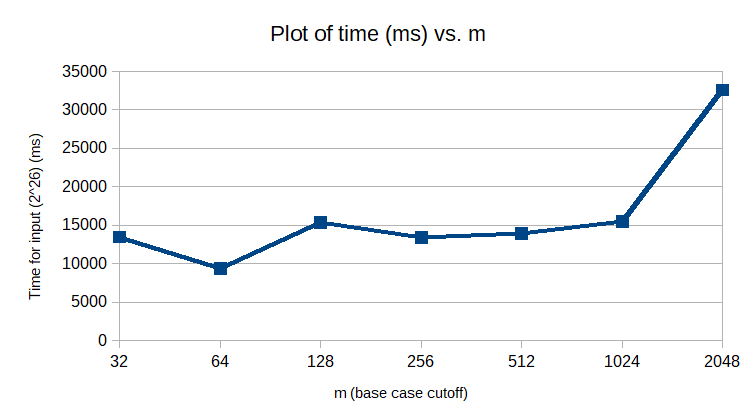
\includegraphics{graph1.png}
    \centering
    \caption{Time (ms) versus. m (base case cutoff) }
\end{figure} 
    
The optimal value obtained is $m = 64$ for this input $n = 67,108,864 $. 

\subsection*{C}

On one processing core, using $m = 64$, we find the largest $n$ such that quicksort runs in under 2 minutes:

\pgfplotstabletypeset[col sep=comma,,
     columns={n, Time (ms) }, fixed,
    ]{task1C_1.csv}
    
Largest value obtained is $n = 268435456  (2^{28})$. We do the same for radix sort:

\pgfplotstabletypeset[col sep=comma,,
     columns={n, Time (ms) }, fixed,
    ]{task1C_2.csv}
    
At this point, the program crashed (perhaps due to memory overload), but the highest was $n =  1073741824 (2^{30})$. The highest value for both implementations is therefore $n = 268435456  (2^{28})$.
We now vary processor cores, and run on both algorithms using the input $n = 268435456  (2^{28})$.

We obtain the following: 

    \begin{figure}[H]
    \centering
    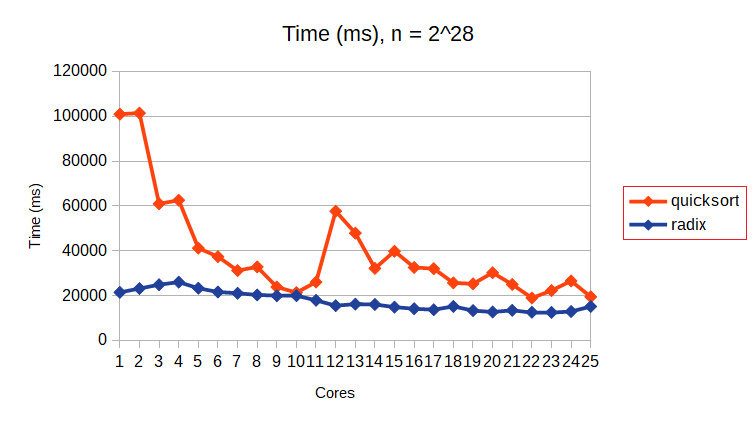
\includegraphics{graph2.png}
    \centering
    \caption{Time (ms) versus. number of cores}
\end{figure} 

\subsection*{D}

Finally, we vary $n$ and measure the running time for both sorting algorithms on all cores. 

   \begin{figure}[H]
    \centering
    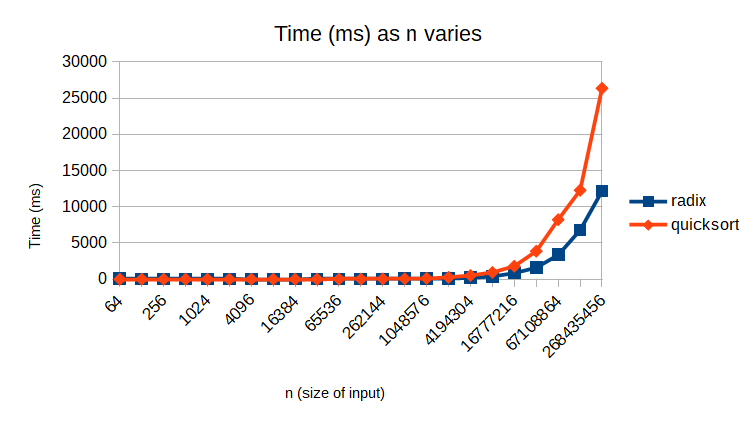
\includegraphics{graph3.png}
    \centering
    \caption{Time (ms) versus. n (input size)}
\end{figure} 

\section*{Task A}

\end{document}